\section{August 2018}

\subsection*{Classical Mechanics}
\addcontentsline{toc}{subsection}{Classical Mechanics}

\prob{1.1}{

A system with two degrees of freedom has the Hamiltonian
\begin{align}
    H = q_1 p_1 - q_2 p_2 - a q_1^2 + b q_2^2
.\end{align}
Determine the constant $c$ so that $F = (p_2 + c q_2)/q_1$ is a constant of motion.

}

\sol{}


\prob{1.2}{

Two equal masses $m$, connected by a massless and inextensible string, hang over two pulleys (of negligible size), as shown in the figure below.
The left mass moves along a vertical line, but the right mass is free to swing back and forth in the plane of the masses and pulleys.

\begin{parts}

\item Use the generalized coordinates shown in the figure, and obtain the Lagrangian.

\item Derive the equations of motion.

\item Obtain the frequency of small oscillations for this system.

\item Assume the left mass starts at rest, and the right mass undergoes small oscillations with angular amplitude $\alpha \ll 1$.
What is the initial acceleration, averaged over a few periods, of the left mass?
In which direction does it move?
    
\end{parts}

\textbf{Hint}: in part (d), you should keep linear and quadratic terms in $\alpha$ and $\dot{\alpha}$ in the equation for $r$.
Also recall that the average of $\cos^2{\phi}$ ($\phi$ is a generic angle) over the interval $[0,2 \pi]$ is $1/2$.

\begin{center}
    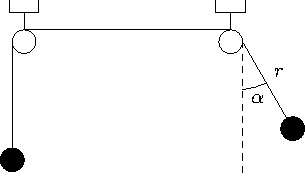
\includegraphics{January2020/1-3.pdf}
\end{center}

}

\sol{}


\prob{1.3}{

Find energy acquired by an undamped oscillator of frequency $\omega_0$ with mass $m$ under the action of the force given by
\begin{align}
    F(t) = \begin{cases}
        F e^{\lambda t} & -\infty < t \leq 0 \\
        F[ 2 - e^{-\lambda t} ] & 0 \leq t < \infty
    ,\end{cases}
\end{align}
where $\lambda > 0$.
At $t = -\infty$, the oscillator was at rest.

}

\sol{}


\prob{1.4}{

A small ball of mass $m$ is connected to a spring of length $L$ and spring constant $k$, the other end of which is attached to the center of a round table.
The table is rotated around its center with a constant angular frequency $\omega$.
Assuming that the ball can only move with no friction in the plane $xy$ of the table,

\begin{parts}

\item write down the Lagrangian and the equations of motion of the ball in the coordinate frame rotating along with the table;

\item calculate the frequencies of small oscillations of the ball;

\item describe the character of motion of the oscillating ball in the rotating coordinate frame.
    
\end{parts}

}

\sol{}


\prob{2.1}{

Two point masses $M$ and $m$ are conected by the (massless and inextensible) rope of length $l$.
The rope is suspended from a small hole in the frictionless table as shown below.
The mass $M$ can move (freely) only up or down while the mass $m$ is free to move on the table surface.

\begin{parts}

\item Write the Lagrangian and Euler-Lagrangian equations for this system.

\item At time $t = 0$ the mass $m$ is at distance $r_0 < l$ from the hole and its velocity is $v_0$ in the direction orthogonal to the rope.
Find at which $v_0$ the motion is circular.

\begin{center}
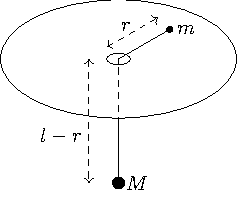
\includegraphics{August2018/2-1.pdf}
\end{center}
    
\end{parts}

}

\subsection*{Electricity \& Magnetism}
\addcontentsline{toc}{subsection}{Electricity \& Magnetism}

\prob{2.2}{

A sphere of radius $R$ is centered at the origin.
The sphere carries a bulk charge density $\rho(r,\theta,\phi)$ and a surface charge density $\sigma(\theta,\phi)$.

Together they produce, in the sphere, the electric field
\begin{align}
    \vb*{E} = -\frac{2 V_0 x}{R^2} \vu*{x} + \frac{2 V_0 y}{R^2} \vu*{y} - \frac{V_0}{R} \vu*{z}
.\end{align}
Determine $\rho(r,\theta,\phi)$ and $\sigma(\theta,\phi)$.

}

\sol{}


\prob{2.3}{

A uniformly charged line segment of length $2a$ centered at the origin and oriented in the $z$-direction is surrounded by a grounded conducting sphere of a radius $R > a$, also centered at the origin.
The total charge on the segment is $q$.

\begin{parts}

\item Find the electrostatic potential inside the sphere.

\item Find the electrostatic potential in the $z = 0$ plane.

\item Find the $\rho \rightarrow 0$ limit of the potential on the $z = 0$ plane, where $\rho = \sqrt{x^2 + y^2}$.
    
\end{parts}

\textbf{Hint}: Useful integral
\begin{align}
    \int \frac{\dd{z}}{\sqrt{z^2 + a^2}} = \ln(z + \sqrt{z^2 + a^2})
.\end{align}

}

\sol{}


\prob{2.4}{

A particle of charge $q$ and mass $m$ moves through an empty space with the velocity $\vb*{v} = v \vu*{x}$ ($v \ll c$).
At time $t = 0$, the uniform magnetic field $\vb*{B} = B \vb*{z}$ is switched on.
How long will it take the particle to lose half of its kinetic energy?
Assume that the magnetic field is sufficiently weak so that the particle loses half of its energy after many revolutions.

}

\sol{}


\prob{3.1}{

An electric dipole $\vb*{d}$ is spaced by the distance $L$ from a plane surface of a metal filling the half space $x < 0$.
Calculate:

\begin{parts}

\item the potential energy $U(L,\theta)$ of the dipole and the interaction force $\vb*{F}(L,\theta)$ between the dipole and the metallic surface as functions of $L$ and the angle $\theta$ between the vector $\vb*{d}$ and the plane of the surface.

\item The torque $\vb*{T} = \vb*{r} \cross \vb*{F}$ acting on the dipole due to its interaction with the surface.
    
\end{parts}

}

\sol{}


\prob{3.2}{

You are going to prove in two steps the mean value theorem: for charge-free space the value of the electrostatic potential at any point is equal to the average of the potential over the surface of any sphere centered on that point, that is
\begin{align}
    \phi(\vb*{r}' = 0) = \frac{1}{4 \pi} \oint \dd{\Omega} \phi(R,\Omega)
,\end{align}
where $R$ is the (arbitrary) radius of the sphere centered at $\vb*{r}'$, taken at the origin of the coordinate system, and the integration in the solid angle $\Omega$ is over the whole $4 \pi$.

Use Green's theorem,
\begin{align}
    \int_V \dd[3]{\vec{r}} &\Big[ \psi_1(\vb*{r}) \laplacian \psi_2(\vb*{r}) - \psi_2(\vb*{r}) \laplacian \psi_1(\vb*{r}) \Big] \nonumber \\
    &= \int_S \dd{S} \vu*{n} \cdot \Big[ \psi_1(\vb*{r}) \grad \psi_2(\vb*{r}) - \psi_2(\vb*(r)) \grad \psi_1(\vb*{r}) \Big]
\end{align}
for the two functions $\psi_1(\vb*{r}) = \phi(\vb*{r})$ and $\psi_2(\vb*{r}) = |\vb*{r} - \vb*{r}'|^{-1}$, where $\phi(\vb*{r})$ is the electrostatic potential, by taking $V$ and $S$ as, respectively, the volume and surface of the sphere of radius $R$.
Show that
\begin{align}
    \phi(\vb*{r}' = 0) = \frac{1}{4 \pi} \oint \dd{\Omega} \phi(R,\Omega) + \frac{R}{4 \pi} \oint \dd{\Omega} \pdv{\phi(r,\Omega)}{r} \Big|_{r = R}
.\end{align}
Use Green's theorem again, but for the functions $\psi_1(\vb*{r}) = \phi(\vb*{r})$ and $\psi_2(\vb*{r}) = 1$, to show that the second integral on the right-hand-side of the equation above vanishes, thus proving the mean value theorem.

}

\sol{}


\prob{3.3}{

Consider an iron sphere of radius $R$ that carries a charge $Q$ and a uniform magnetization $\vb*{M} = M \vu*{z}$.
What is the angular momentum stored in the electromagnetic fields if the sphere is at rest?

}

\subsection*{Quantum Mechanics}
\addcontentsline{toc}{subsection}{Quantum Mechanics}


\prob{3.4}{

Consider a particle of mass $m$ placed in an infinite two-dimensional potential well with a width $a$:
\begin{align}
    V(x,y) = \begin{cases}
        0 & 0 \leq x,y \leq a \\
        \infty & {\rm otherwise}
    .\end{cases}
\end{align}
The particle is also subject to a perturbation $W$ described by the potential
\begin{align}
    W(x,y) = \begin{cases}
        w_0 & 0 \leq x,y \leq \frac{a}{2} \\
        \infty & {\rm otherwise}
    .\end{cases}
\end{align}

\begin{parts}

\item Calculate to first order in $w_0$ the perturbed energy of the ground state.

\item Calculate to first order in $w_0$ the perturbed energies of the first excited states.
Give the corresponding wave functions to zeroth order in $w_0$.

\end{parts}

}

\sol{



}


\prob{4.1}{

The Hamiltonian for a particle of mass $m$ moving in a three-dimensional space is
\begin{align}
    H = \frac{p_x^2 + p_y^2 + p_z^2}{2m} + \lambda x
.\end{align}
Find $\expval{L_x}$ as a function of time if, at $t = 0$
\begin{align}
\begin{aligned}
    \expval{L_x} &= a, \\
    \expval{y} &= b, \\
    \expval{p_y} &= c
,\end{aligned}
\end{align}
where $\lambda$, $a$, $b$, and $c$ are constants.

}

\sol{

Recall the Ehrenfest theorem:
\begin{align}
    \dv{\expval{L_x}}{t} = \frac{i}{\hbar} \expval{[H,L_x]}
.\end{align}
The commutator
\begin{align}
    [H,L_x] = \frac{1}{2m} \Big( [p_x^2,L_x] + [p_y^2,L_x] + [p_z^2,L_x] \Big) + \lambda [x,L_x]
\end{align}
Recalling that $[V_i,L_j] = i \hbar \epsilon_{ijk} V_k$, where $\vec{V}$ is a vector operator, we have
\begin{align}
    [p_i^2,L_x] = p_i [p_i,L_x] + [p_i,L_x] p_i = i \hbar \epsilon_{i1k} ( p_i p_k + p_k p_i ) = 2 i \hbar \epsilon_{i1k} p_i p_k
\end{align}
and
\begin{align}
    [x,L_x] = i \hbar \epsilon_{11k} r_k = 0
.\end{align}
Putting this into the relevant commutator, we find
\begin{align}
    [H,L_x] = \frac{1}{2m} \Big( - 2 i \hbar p_y p_z + 2 i \hbar p_z p_y  \Big) = 0
.\end{align}
We have therefore found that $L_x$ commutes with the Hamiltonian, implying that 
\begin{align}
    \dv{\expval{L_x}}{t} = 0 \Rightarrow \eqbox{ \expval{L_x(t)} = a }
.\end{align}

}


\prob{4.2}{

Consider a system of spin-1/2.
What are the eigenstates and eigenvalues of the operator $S_x + S_y$?
Suppose a measurement of this quantity is made, and the system is found to be in the eigenstate with the larger eigenvalue.
What is the probability that a subsequent measurement of $S_y$ yields $\hbar/2$?

}

\sol{

We can write $S_x + S_y = (\hbar/2) (\sigma_x + \sigma_y)$.
The matrix representation of the sum of Pauli matrices
\begin{align}
    \sigma_x + \sigma_y = \begin{pmatrix}
        0 & 1 - i \\
        1 + i & 0
    \end{pmatrix}
,\end{align}
which we can diagonalize in the usual way, yielding eigenvalues $\pm \sqrt{2}$ with corresponding eigenvectors 
\begin{align}
\chi_{\pm} = \frac{1}{\sqrt{2}} \begin{pmatrix} 1 \\ \pm (1 + i) / \sqrt{2} \end{pmatrix}    
.\end{align}
If we take a measurement of the system and find it to be in the eigenstate $\chi_+$, then the probability a subsequent measurement of $S_y$ will yield $\hbar/2$ is given by
\begin{align}
    P &= |\ip{+_y}{\chi_+}|^2 = \frac{1}{4} \Big| \begin{pmatrix}
        1 & -i
    \end{pmatrix} \begin{pmatrix}
        1 \\ (1+i)/\sqrt{2}
    \end{pmatrix} \Big|^2 \nonumber \\
    &= \frac{1}{4} | 1 - (-i + 1) / \sqrt{2} |^2 = \frac{1}{4} \Big[ (1 - 1/\sqrt{2})^2 + 1 \Big] \nonumber \\
    &= \eqbox{ \frac{5 - 2 \sqrt{2}}{8} \approx \frac{1}{4} }
\end{align}


}


\prob{4.3}{

At time $t = 0$, the state of a free one-dimensional particle is described by the wave function
\begin{align}
    \Psi(x,t=0) = A \exp[ -\frac{x^2}{2a^2} + i \frac{m v_0 x}{\hbar} ]
.\end{align}

\begin{parts}

\item Find the wave function at arbitrary time $t$.

\item Find the averages $\expval{x(t)}$ and $\expval{p(t)}$.
    
\end{parts}

}

\sol{

(a) There are a couple ways to obtain the answer.
Let's use the unitary time evolution operator:
\begin{align}
    \ket{\Psi(t)} = e^{-i H t / \hbar} \ket{\Psi(0)}
.\end{align}
Since our particle is free, the Hamiltonian $H = p^2 / 2m$, so our Hamiltonian eigenstates are also momentum eigenstates.
It is convenient then to expand in these states:
\begin{align}
    \ket{\Psi(t)} = e^{-i H t / \hbar} \int \dd{p} \ket{\psi_{p}} \ip{\psi_p}{\Psi(0)} = \int \dd{p} e^{-i E t / \hbar} \ket{\psi_p} \ip{\psi_p}{\Psi(0)}
,\end{align}
and projecting onto the position states, we have
\begin{align}
    \Psi(x,t) &= \ip{\phi_x}{\Psi(t)} = \int \dd{p} e^{-i E t / \hbar} \ip{\phi_x}{\psi_p} \Bigg[ \int \dd{x} \ip{\psi_p}{\phi_x} \ip{\phi_x}{\Psi(0)} \Bigg] \nonumber \\
    &= \int \frac{\dd{p}}{\sqrt{2 \pi \hbar}} e^{i(px - Et) / \hbar} \underbrace{ \Bigg[ \int \frac{\dd{x}}{\sqrt{2 \pi \hbar}} e^{-i p x / \hbar} \Psi(x,0) \Bigg] }_{\widetilde{\Psi}(p,0)}
.\end{align}
From this, we can see that we must compute the Fourier transform of our initial wave-function.
First, we compute the normalization:
\begin{align}
    1 = A^2 \int _{-\infty}^{\infty} \dd{x} e^{-x^2/a^2} = A^2 \sqrt{\pi} a \Rightarrow A = (\pi a^2)^{-1/4}
\end{align}
\begin{align}
    \widetilde{\Psi}(p,0) &= (\pi a^2)^{-1/4} \int_{-\infty}^{\infty} \frac{\dd{x}}{\sqrt{2 \pi \hbar}} e^{-i p x / \hbar} e^{-x^2/2a^2 + i m v_0 x / \hbar} \nonumber \\
    &= \Big( 4 \pi^3 a^2 \hbar^2 \Big)^{-1/4} \int_{-\infty}^{\infty} \dd{x} e^{i(mv_0 - p) x / \hbar} e^{-x^2/2a^2}
.\end{align}
We will need the following generic integral:
\begin{align}
    \int_{-\infty}^{\infty} \dd{x} e^{i \beta x} e^{-x^2/(2 \sigma^2)} &= \int_{-\infty}^{\infty} \dd{x} e^{-[x^2 - 2 i \sigma^2 \beta x]/(2\sigma^2)} = \int_{-\infty}^{\infty} \dd{x} e^{-[(x - i \sigma^2 \beta)^2 - (-i \sigma^2 \beta)^2]/(2 \sigma^2)} \nonumber \\
    &= \sigma \sqrt{2 \pi} e^{-\sigma^2 \beta^2 / 2}
.\end{align}
Using this, we have
\begin{align}
    \widetilde{\Psi}(p,0) = \Big( \frac{a^2}{\pi \hbar^2} \Big)^{1/4} e^{-a^2(p - mv_0)^2/(2\hbar^2)}
.\end{align}

Next, we can compute the time-dependence of the state:
\begin{align}
    \Psi(x,t) &= \frac{1}{\sqrt{2 \pi \hbar}} \Big( \frac{a^2}{\pi \hbar^2} \Big)^{1/4} \int_{-\infty}^{\infty} \dd{p} e^{i(px - p^2 t / (2m)) / \hbar} e^{-a^2(p - m v_0)^2 / (2\hbar^2)} \nonumber \\
    &= \Big( \frac{a^2}{4 \pi^3 \hbar^4} \Big)^{1/4} e^{-a^2 m^2 v_0^2 / (2 \hbar^2)} \int_{-\infty}^{\infty} \dd{p} e^{i[ x / \hbar - 2 i a^2 m v_0 / (2 \hbar^2) ] p} e^{-[a^2/\hbar^2 + i t / (m\hbar)] p^2 / 2} \nonumber \\
    &= \Big( \frac{a^2}{4 \pi^3 \hbar^4} \Big)^{1/4} e^{-a^2 m^2 v_0^2 / (2 \hbar^2)} \sqrt{\frac{2 \pi m \hbar^2}{m a^2 + i \hbar t}} e^{-[x/\hbar - i a^2 m v_0/\hbar^2]^2 / \{ 2 [a^2 / \hbar^2 + i t / (m \hbar)] \}} \nonumber \\
    &= \eqbox{ \frac{1}{\sqrt{ma^2 + i \hbar t}} \Big( \frac{m^2 a^2}{\pi} \Big)^{1/4} e^{-a^2 m^2 v_0^2 / (2 \hbar^2)} e^{-m (x - i a^2 m v_0 / \hbar)^2/[ 2 (ma^2 + i \hbar t) ]} }
.\end{align}
Thankfully, we are done.
As a sanity check, we should check that this matches our initial condition:
\begin{align}
    \Psi(x,0) &= \frac{1}{\sqrt{ma^2}} \Big( \frac{m^2 a^2}{\pi \hbar^2} \Big)^{1/4} e^{-a^2 m^2 v_0^2 / (2 \hbar^2)} e^{-[x - i a^2 m v_0 / \hbar]^2/(2a^2)} \nonumber \\
    &= ( \pi a^2 )^{-1/4} e^{-x^2/2a^2 + i m v_0 x / \hbar}
.\end{align}


(b) In this part, we are supposed to compute expectation values of the position and momentum.
The calculation for the position expectation value is as follows:
\begin{align}
\eqbox{
\begin{aligned}    
    \expval{x} &= \int_{-\infty}^{\infty} \dd{x} x |\Psi(x,t)|^2 \sqrt{ \frac{m^2a^2}{\pi( m^2 a^4 + \hbar^2 t^2)}} \int_{-\infty}^{\infty} \dd{x} x e^{-m^2 a^2 (x - v_0 t)^2/(m^2a^4 + \hbar^2 t^2)} \nonumber \\
    &= v_0 t
\end{aligned}
}
.\end{align}
This was a very long-winded way of saying that the center of the wave packet moves with velocity $v_0$ to the right.

Next, we can avoid taking derivatives of this nasty Gaussian by making use of the Ehrenfest theorem, which states that
\begin{align}
    \dv{\expval{p}}{t} = \frac{i}{\hbar} \expval{[H,p]} = 0
.\end{align}
Thus, the average value of $p$ is constant, and we need only know the initial average value:
\begin{align}
    \eqbox{ \expval{p} = \int_{-\infty}^{\infty} \dd{p} p |\widetilde{\Psi}(p,0)|^2 = m v_0 }
,\end{align}
since the Gaussian is even about $m v_0$.

Note that we could have obtained the expectation value of $x$ a bit simpler using the Ehrenfest theorem too:
\begin{align}
    \dv{\expval{x}}{t} = \frac{i}{\hbar} \expval{[H,x]} = \frac{i}{2 m \hbar} \expval{[p^2,x]} = \frac{i}{2m \hbar} \expval{-2i\hbar p} = \frac{\expval{p}}{m} = v_0
.\end{align}
Thus,
\begin{align}
    \expval{x} = v_0 t
,\end{align}
where the initial average position is just zero since the Gaussian is centered there.

}


\prob{4.4}{

Consider the Hamiltonian of two interacting oscillators:
\begin{align}
    H = \hbar \omega [ a^{\dagger} a + b^{\dagger} b + k( a^{\dagger} b + b^{\dagger} a ) + 1 ]
\end{align}
where $a$ and $b$ are the ladder operators for the oscillator 1 and 2 satisfying the bosonic commutation relations $[a^{\dagger},a] = 1$ and $[b^{\dagger},b] = 1$, and $k$ is a dimensionless coupling constant.

\begin{parts}

\item Diagonalize $H$ using the unitary transformation
\begin{align}
    a = \alpha \cos{\theta} + \beta \sin{\theta}, \quad b = \beta \cos{\theta} - \alpha \sin{\theta}
.\end{align}

\item Show that the new operators $\alpha$ and $\beta$ satisfy the same commutation relations $[\alpha,\alpha^{\dagger}] = 1$ and $[\beta,\beta^{\dagger}] = 1$ as $a$ and $b$.

\item Calculate the energy levels for the oscillators.
    
\end{parts}

}

\sol{

(a) We introduce the new operators $\alpha$, $\beta$ as prescribed (the transformation is reminiscent of normal coordinates in classical mechanics which act as independent oscillators), allowing us to write
\begin{align}
    a^{\dagger} a &= (\alpha^{\dagger} \cos{\theta} + \beta^{\dagger} \sin{\theta})(\alpha \cos{\theta} + \beta \sin{\theta}) \nonumber \\
    &= \alpha^{\dagger} \alpha \cos^2{\theta} + ( \alpha^{\dagger} \beta + \beta^{\dagger} \alpha ) \cos{\theta} \sin{\theta} + \beta^{\dagger} \beta \sin^2{\theta} \\
%
    b^{\dagger} b &= (\beta^{\dagger}\cos{\theta} - \alpha^{\dagger} \sin{\theta})(\beta\cos{\theta} - \alpha \sin{\theta}) \nonumber \\
    &= \beta^{\dagger} \beta \cos^2{\theta} - (\beta^{\dagger}\alpha + \alpha^{\dagger} \beta) \cos{\theta} \sin{\theta} + \alpha^{\dagger} \alpha \sin^2{\theta} \\
%
    a^{\dagger} b &= (\alpha^{\dagger} \cos{\theta} + \beta^{\dagger} \sin{\theta}) (\beta \cos{\theta} - \alpha \sin{\theta}) \nonumber \\
    &= (\beta^{\dagger} \beta - \alpha^{\dagger} \alpha) \cos{\theta} \sin{\theta} + \alpha^{\dagger} \beta \cos^2{\theta} - \beta^{\dagger} \alpha \sin^2{\theta}
.\end{align}
In terms of $\alpha$ and $\beta$, the Hamiltonian
\begin{align}
    H = \hbar \omega \Big[ \alpha^{\dagger} \alpha + \beta^{\dagger} \beta + k [ 2(\beta^{\dagger} \beta - \alpha^{\dagger} \alpha) \cos{\theta}\sin{\theta} + (\alpha^{\dagger} \beta - \beta^{\dagger} \alpha ) (\cos^2{\theta} - \sin^2{\theta}) ] + 1 \Big]
.\end{align}
If we choose $\theta = \pi/4$, then $\cos{\theta} = \sin{\theta} = 1/\sqrt{2}$, and
\begin{align}
    \eqbox{ H = \hbar \omega \Big[ (1 - k) \alpha^{\dagger} \alpha + (1 + k) \beta^{\dagger} \beta + 1 \Big] }
.\end{align}
Notice that we have effectively diagonalized our Hamiltonian.
That is, if we know the eigenstates of $\alpha^{\dagger} \alpha$ and $\beta^{\dagger} \beta$ (which we may posit are number operators at the moment and will be proven in the next part), then the eigenstates of this Hamiltonian are simply tensor products of these. 

(b) Observe that we can invert the transformation used in part (a) to write
\begin{align}
    \alpha &= \frac{1}{\sqrt{2}} (a - b), \quad \beta = \frac{1}{\sqrt{2}} (a + b)
.\end{align}
The commutators
\begin{align}
\eqbox{
\begin{aligned}
    [\alpha,\alpha^{\dagger}] &= \frac{1}{2} [a-b,a^{\dagger}-b^{\dagger}] = \frac{1}{2} \Big( \underbrace{ [a,a^{\dagger}] }_{=1} - \underbrace{ [a,b^{\dagger}] }_{=0} - \underbrace{ [b,a^{\dagger}] }_{=0} + \underbrace{ [b,b^{\dagger}] }_{=1} \Big) = 1 \\
    [\beta,\beta^{\dagger}] &= \frac{1}{2} [a+b,a^{\dagger}+b^{\dagger}] = \frac{1}{2} \Big( [a,a^{\dagger}] + [a,b^{\dagger}] + [b,a^{\dagger}] + [b,b^{\dagger}] \Big) = 1
\end{aligned}
}
.\end{align}
Thus, the operators $\alpha$, $\alpha^{\dagger}$ and $\beta$, $\beta^{\dagger}$ are lowering and raising operators for independent oscillators with number operator spectra $\alpha^{\dagger} \alpha \ket{n_{\alpha}} = n_{\alpha} \ket{n_{\alpha}}$ and $\beta^{\dagger} \beta \ket{n_{\beta}} = n_{\beta} \ket{n_{\beta}}$.

(c) From the previous parts, we observe that the eigenstates of the Hamiltonian are the tensor product states $\ket{n_{\alpha},n_{\beta}} = \ket{n_{\alpha}} \otimes \ket{n_{\beta}}$ with corresponding eigenvalues
\begin{align}
    \eqbox{ E_{n_{\alpha},n_{\beta}} = \hbar \omega \big[ (1-k) n_{\alpha} + (1+k) n_{\beta} + 1 \big] }
.\end{align}

}
